\documentclass[tikz]{standalone}
\usepackage{pgfplots}

\pgfplotsset{compat=newest}
\pgfplotsset{
    yticklabel style={
        /pgf/number format/fixed,
        /pgf/number format/precision=2
    },
    scaled y ticks=false
}

\begin{document}
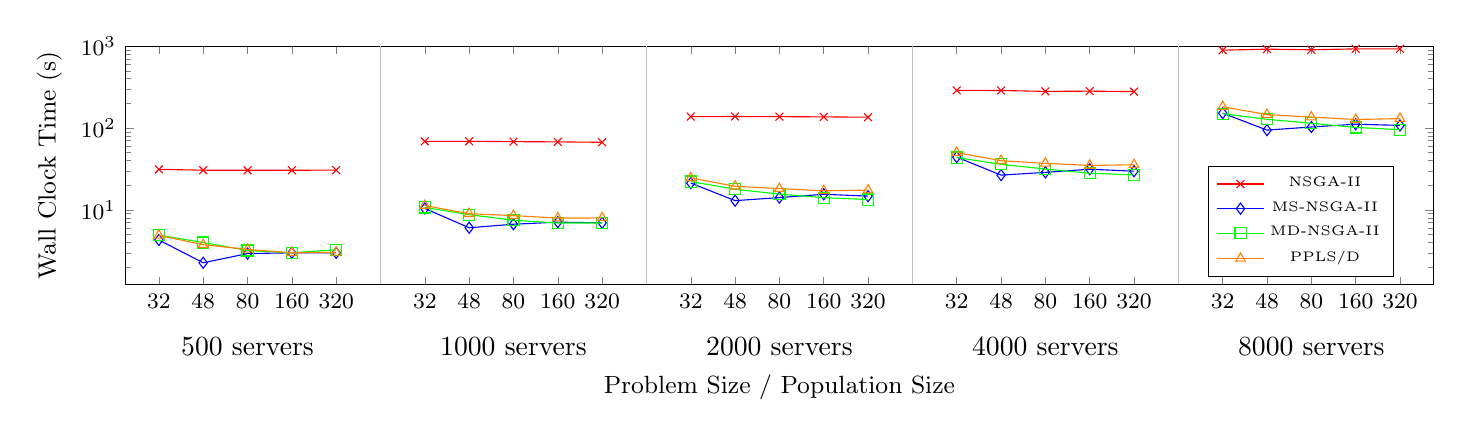
\begin{tikzpicture}

    \begin{axis}[
        footnotesize,
        max space between ticks=20pt,
        width=1.5\textwidth,
        height=0.38\textwidth,
        ymax = 1000,
        try min ticks=5,
        xtick=data,
        xticklabels={32, 48, 80, 160, 320, 32, 48, 80, 160, 320, 32, 48, 80, 160, 320, 32, 48, 80, 160, 320, 32, 48, 80, 160, 320},
        extra x ticks={5,11,17,23},
        extra x tick labels={},
        extra x tick style={
            grid=major,
            major tick length=0pt,
        },
        xlabel={Problem Size / Population Size},
        ylabel={Wall Clock Time (s)},
        xlabel style={
            yshift=-4ex,
        },
        enlarge x limits={abs=0.75},
        legend pos=south east,
        legend entries={
            {NSGA-II},
            {MS-NSGA-II},
            {MD-NSGA-II},
            {PPLS/D},
        },
        clip mode=individual,
        legend style={font=\tiny},
        ymode=log
    ]

    \addplot[
        mark=x,
        color=red
    ] table[
        x expr=\coordindex,
        y=TM
    ]{
        PS TM
        32 31.3333
        48 30.6
        80 30.5
        160 30.5333
        320 30.6667
        {} {}
        
        32 68.9
        48 68.9
        80 68.2667
        160 67.8333
        320 67
        {} {}
        
        32 138
        48 138.2667
        80 137.9
        160 136.9333
        320 135.7
        {} {}
        
        32 288.5
        48 287.6333
        80 280.2667
        160 282.2333
        320 278.8333
        {} {}
        
        32 892.4333
        48 919.2
        80 903
        160 926.4
        320 926.6
        {} {}         
    };

    \addplot[
        mark=diamond,
        color=blue
    ] table[
        x expr=\coordindex,
        y=TM
    ]{
        PS TM
        32 4.3
        48 2.2667
        80 2.9333
        160 3
        320 3
        {} {}
        
        32 10.4333
        48 6.0667
        80 6.7
        160 7.1
        320 6.9667
        {} {}
        
        32 21.3
        48 13
        80 14.1667
        160 15.5333
        320 14.7667
        {} {}
        
        32 44.2
        48 26.6333
        80 28.7667
        160 31.4667
        320 29.7333
        {} {}
        
        32 152.2
        48 94.4333
        80 103.0667
        160 111.4333
        320 107.8
        {} {}          
    };

    \addplot[
        mark=square,
        color=green
    ] table[
        x expr=\coordindex,
        y=TM
    ]{
        PS TM
        32 4.9333
        48 4
        80 3.2
        160 3
        320 3.2667
        {} {}
        
        32 10.7333
        48 8.7667
        80 7.5
        160 6.9333
        320 6.9333
        {} {}
        
        32 22.2333
        48 17.9
        80 15.6333
        160 14.1333
        320 13.4
        {} {}
        
        32 43.6667
        48 36.0667
        80 31.6
        160 28.0667
        320 26.7667
        {} {}
        
        32 149.8667
        48 127.9667
        80 114.4
        160 101.7667
        320 95.6333
        {} {}          
    };

    \addplot[
        mark=triangle,
        color=orange
    ] table[
        x expr=\coordindex,
        y=TM
    ]{
        PS TM
        32 4.9
        48 3.7667
        80 3.3
        160 3
        320 3.0333
        {} {}
        
        32 11.3333
        48 9
        80 8.5333
        160 7.9667
        320 8
        {} {}
        
        32 24.6
        48 19.4667
        80 18.2333
        160 17.1333
        320 17.4667
        {} {}
        
        32 50.2333
        48 39.9667
        80 37.0667
        160 34.9667
        320 35.6333
        {} {}
        
        32 182.1333
        48 145.9333
        80 136.3333
        160 127.1667
        320 130.5
        {} {}            
    };

    \begin{scope}[
        every label/.append style={
            label distance=2ex,
        },
    ]
        \node [label=below:500 servers, yshift=4.5ex]
            at (axis cs:2,\pgfkeysvalueof{/pgfplots/ymin}) {};
        \node [label=below:1000 servers, yshift=4.5ex]
            at (axis cs:8,\pgfkeysvalueof{/pgfplots/ymin}) {};
        \node [label=below:2000 servers, yshift=4.5ex]
            at (axis cs:14,\pgfkeysvalueof{/pgfplots/ymin}) {};
        \node [label=below:4000 servers, yshift=4.5ex]
            at (axis cs:20,\pgfkeysvalueof{/pgfplots/ymin}) {};
        \node [label=below:8000 servers, yshift=4.5ex]
            at (axis cs:26,\pgfkeysvalueof{/pgfplots/ymin}) {};
    \end{scope}
    \end{axis}
\end{tikzpicture}
\end{document}